\section{Method}
\label{sec:metodo}

In order to build the knowledge graph of the semantic relationships between 
the objects found in a certain close environment of human occupation, such as 
a room, a deductive database \cite{stichbury}, we used Grakn.
% Para construir el grafo de conocimiento de las relaciones semánticas entre 
% los objetos que se encuentran en un determinando ambiente cerrado de ocupación 
% humana, como una habitación, se utilizó una base de datos deductiva 
% \cite{stichbury}, mejor conocida como Grakn.

Grakn is an Open Source engine for creating knowledge graphs that allow the 
user to organize and model complex data networks using the Entity-Relationship 
scheme in its maximum expressiveness. The architecture of Grakn is basically 
made up of two parts, as shown in Figure \ref{fig:arch}: \textit{Grakn} 
(the storage) and \textit{Graql} (the language).
% Grakn es un motor Open Source para la creación de grafos de conocimiento 
% que permite al usuario organizar y modelar redes complejas de datos por medio 
% del esquema Entidad-Relación en su máxima expresividad. La arquitectura de 
% Grakn se compone básicamente de dos partes como observa en la Figura 
% \ref{fig:arch}: \textit{Grakn} (el almacenamiento) y \textit{Graql} 
% (el lenguaje).

\begin{figure}[H]
    \centering
    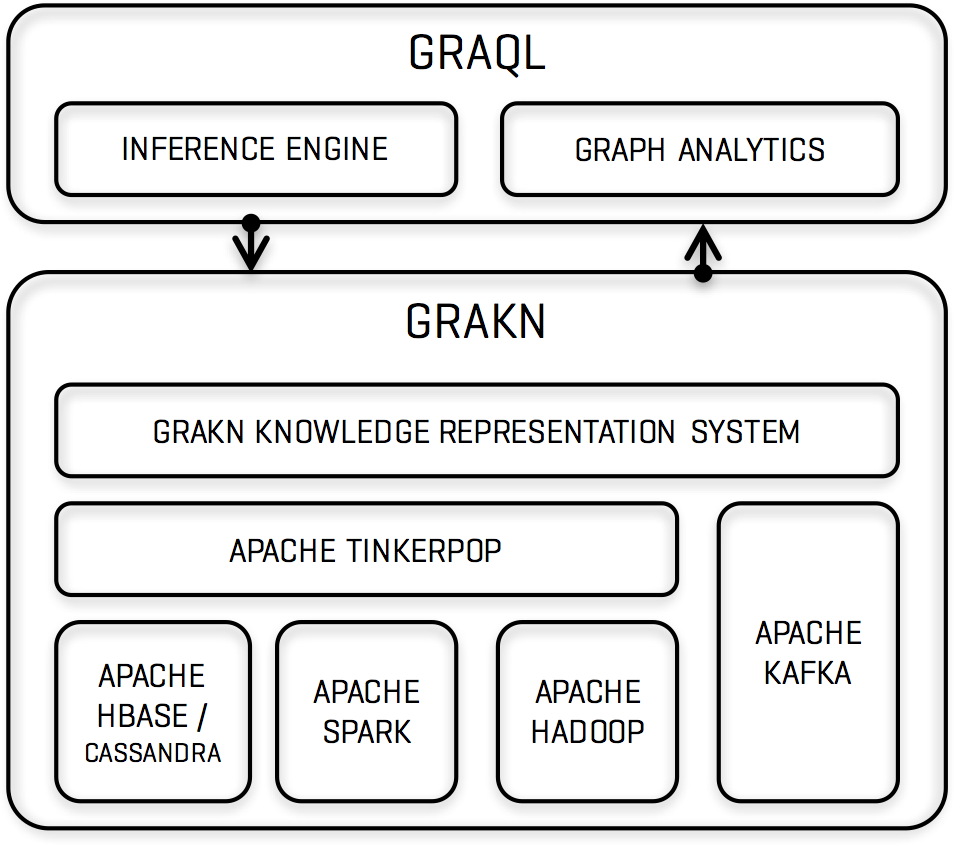
\includegraphics[width=6.8cm]{figures/architecture}
    % \caption{Arquitectura interna de Grakn.
    % Fuente \cite{stichbury}.}
    \caption{Internal architecture of Grakn.
    Source \cite{stichbury}.}
    \label{fig:arch}
\end{figure}

In general, \textit{Grakn} can be seen as a distributed, hyper-relational 
database that uses intuitive\footnote{Refers to the definition of types, 
properties and relationships between existing entities in a given context.} 
ontology\footnote{It should not be seen from the side of philosophy, but as a 
branch of computer science.}  to model complex data, which serves as a 
knowledge base for cognitive systems \cite{dbengines}. 
%% Fig description
In figure \ref{fig:arch}, at the bottom we can see the Grakn system layer, 
which is made of Apache technologies: %
i) \textit{HBase}\footnote{Cassandra database servers the same purposes. It is 
a non-relational database that is distinguished by its speed, scale, 
and simplicity in design.} is a distributed, scalable, big data store databse, 
ii) \textit{Spark} for distributed processing system used for 
big data workloads.
iii) \textit{Hadoop} allows us to hanlde distributed processing of large data 
sets across clusters of computers using simple programming models.
This 3 technologies are the tools for \textit{Tinkerpop} to create the graph 
structure. At the right side of figure \ref{fig:arch} we have \textit{Kafka},
and its main function is to help the Grakn software to make graph data analytics
On the other hand, at the top of figure \ref{fig:arch} we have
\textit{Graql},it can be seen as a wrapper or friendly interface of the Grakn
system layer. Formaly, it is a knowledge-oriented declarative graph query 
language that retrieves knowledge in a explicit or implicit way.
% De manera general, se puede ver a \textit{Grakn} como una base de datos 
% distribuida, hiper-relacional que utiliza una  ontología\footnote{No debe 
% verse desde el lado del la filosofía, sino como una rama de las ciencias de 
% la computación} intuitiva\footnote{se refiere a la definicion de tipos, 
% propiedades y relaciones entre entidades existentes en un determinado 
% contexto} para modelar datos complejos, que sirve como base de conocimiento 
% para los sistemas cognitivos \cite{dbengines}. Por otra parte, \textit{Graql} 
% es un lenguaje de consulta de grafos declarativo orientado al conocimiento 
% (Knowledge-oriented) que recupera conocimiento de manera explícita.

Grakn was designed to be integrated with other technologies that allow it to 
function in a distributed manner. In addition, it is a great complement to 
Natural Language Processing (NLP) and Machine Learning (ML) systems 
\cite{grakn-youtube}.
% Grakn esta diseñado para su integración con otras tecnologías que le permitan 
% funcionar de manera distribuida. Además, es un gran complemento para sistemas 
% de Natural Languaje Processing (NLP) y Machine Learning (ML) 
% \cite{grakn-youtube}. También es importante destacar que los datos son 
% almancenados en Apache Cassandra, una base de datos no relacional que se 
% distingue por su rapidez, escalamiento horizontal y simplicidad en el diseño.

Since Grakn creation in 2016 to present-day, it is use by several international 
companies, such as: Google and Cisco; and by institutions like MIT, OpenCTI, 
and Cares Genetics. Table \ref{fig:grakn-car} summarizes the most important 
features reported by the db-engines \cite{dbengines} site. A more detailed 
explanation can be found on the official Grakn site (\url{https://grakn.ai/}).
% Grakn desde su creación en 2016 hasta la fecha es utilizada por varias 
% trasnacionales, como: Google y Cisco; y por instituciones como MIT, OpenCTI 
% y Cares Genetics. La Tabla \ref{fig:grakn-car} resume las características 
% más importantes que reporta el sitio db-engines \cite{dbengines}. Una 
% explicación con mayor detalle se puede encontrar en el sitio oficial de 
% Grakn (\url{https://grakn.ai/}).

\begin{table}[H]
% \caption{Característica principales de Grakn}
\caption{Grakn main features}
\begin{adjustbox}{width=\columnwidth,center}
\begin{tabular}{|l|l|}
\hline
\textbf{Feature}             & \textbf{Description}                   \\ \hline
% \textbf{Característica}             & \textbf{Descripción}          \\ \hline
Database model                      & Graph DBMS  and relational DBMS \\ \hline
% Modelo de base de datos     & DBMS que usa Grafos y DBMS relacional \\ \hline
Initial release                     & 2016                            \\ \hline
% Lanzamiento inicial                 & 2016                          \\ \hline
Current version                     &  1.7.2, June 2020            \\ \hline
% Versión actual                      & 1.7.2, Junio de 2020          \\ \hline
Origin country                      & United Kingdom               \\ \hline
% País de origen                      & Reino Unido                   \\ \hline
License                             & Open Source                  \\ \hline
% Licencia                            & Open Source                   \\ \hline
Implementing language               & Java                         \\ \hline
% Lenguaje de implementación          & Java                          \\ \hline
Supporting operative systems        & Linux, OS X and Windows      \\ \hline
% Sistemas operativos soportados      & Linux, OS X y Windows         \\ \hline
Triggers                            & no                            \\ \hline
Supporting languages                & 
\begin{tabular}[c]{@{}l@{}}All languages base on JVM:
\\ Groovy,\\ Java,\\ JavaScript (Node.js),\\ Python,\\Scala\end{tabular}\\\hline
% Lenguaje de programación soportados & 
% \begin{tabular}[c]{@{}l@{}}Todos los lenguajes 
% basados en JVM:\\ Groovy,\\ Java,\\ JavaScript (Node.js),\\ Python,\\ 
% Scala\end{tabular} \\ \hline
APIS and other access methods       & 
\begin{tabular}[c]{@{}l@{}}Console (shell),\\ 
gRPC protocol,\\ Workbase (visualisation software)\end{tabular}      \\ \hline
% APIs y otros métodos de acceso      & 
% \begin{tabular}[c]{@{}l@{}}console (shell),\\ 
% gRPC protocol,\\ Workbase (visualisation software)\end{tabular}     \\ \hline
Technical docs                      & https://dev.grakn.ai/­doc         \\ \hline
% Documentación técnica               & https://dev.grakn.ai/­doc  \\ \hline
Usually compare with                & Neo4j, GraphDB y JanusGraph     \\ \hline
% Se compara usualmente con           & Neo4j, GraphDB y JanusGraph   \\ \hline
\end{tabular}
\end{adjustbox}
\label{fig:grakn-car}
\end{table}

\subsection{Grakn installation} % (fold)
% \subsection{Instalación de Grakn} % (fold)

To install Grakn, Java 8 SDK is previously required, if not you can download 
Oracle or OpenJDK implementation. To install Grakn in Linux we can use three 
package managers: \texttt{dnf}, \texttt{yum} (for systems that uses RPM
\footnote{RPM is a recursive acronym which means RPM Package Manager}) 
and \texttt{apt}.
% Para la instalación de Grakn se necesita tener previamente instalado Java 8, 
% en caso de no tenerlo, se puede utilizar la versión proporcionada por Oracle 
% o por OpenJDK. En el caso de Linux, la instalación de Grakn puede hacerse a 
% través de tres gestores de paquetes: \texttt{dnf}, \texttt{yum} (para sistemas 
% que usen gestores RPM\footnote{RPM es un acrónimo recursivo que se desglosa 
% como RPM Package Manager}) y \texttt{apt}.

Besides, Grakn is also available for X OS operative system,  through 
\texttt{brew} package manager. The testing implementations presented in the 
paper were made using CentOS 8.2 and Manjaro Linux 20.0.
% Además, Grakn está disponible también para los sistemas operativos X OS, a 
% través del gestor de paquetes \texttt{brew}. Para este proyecto con el fin de 
% realizar las pruebas de implementación se utilizaron CentOS 8.2 y Manjaro 
% Linux 20.0.

Another important point is that Grakn works similarly to database management 
systems, which means we must start services, create users, workspaces, 
among others. In Grakn the abstract models that encapsulate 
the entities of a particular problem are known as \textit{Keyspace}, where the 
\textit{schemes} that will represent the data of the case study are defined.
% Es importante destacar que Grakn funciona de manera similar a los sistemas 
% manejadores de base de datos, es decir, se deben iniciar servicios, crear 
% usuarios, crear espacios de trabajo, entre otros. En Grakn los modelos 
% abstractos que encapsulan y las entidades de un problema en particular 
% son conocidos como \textit{Keyspace}, donde se definen los \textit{esquemas} 
% que representarán los datos del caso de estudio.

An \textit{scheme} is an inherent part of the knowledge graph that describes 
what data is like and how it can be structured. It can be represented by an 
Entity-Relationship diagram. On the other side, Grakn has various types that 
made up the core system and provide the vocabulary necessary to describe any 
case study. The most important Grakn data types are:
% Un \textit{esquema} es un parte inherente del grafo de conocimiento que 
% describe cómo son los datos y cómo pueden ser estructurados. Dicho esquema 
% se puede representar por medio de un diagrama entidad-relación. En Grakn 
% existen tipos que constituyen el núcleo del esquema y proporcionan el 
% vocabulario necesario para describir cualquier caso de estudio. Entre los 
% principales tipos que maneja Grakn destacan:

\begin{itemize}
    \item \textit{Entities}. They provide the means to classify the objects of 
    a given domain.
    % \item \textit{Entidades}. Proveen los medios para clasificar los 
    % objetos de un dominio.
    \item \textit{Relationships}. They connect the elements, known in Grakn as 
        \textit{things} from a particular domain. They can be objects, 
        relationships y attributes.
    % \item \textit{Relaciones}. Conectan los elementos, conocidos en Grakn 
        % como \textit{things}) de un dominio. Estos pueden ser: objetos, 
        % relaciones y atributos.
    \item \textit{Attributes}. They describe the entities.
    % \item \textit{Atributos}. Son usados para caracterizar las entidades.
\end{itemize}

Likewise, it is important to mention that the query language \textit{Graql} 
has the following characteristics:
% Asimismo, es importante mencionar que el lenguaje de consultas \textit{Graql} 
% presenta las siguientes características, mismas que fueron de utilidad para 
% este trabajo.

\begin{itemize}
    \item \textit{Declarative}. In order to make a query with Graql, it may 
        describe what you want to recover, instead of saying how it should be 
        obtained.
    % \item \textit{Declarativo}. Para hacer una consulta con Graql se tiene 
        % describir lo que se quiere recuperar, en lugar de decir 
        % cómo se debe obtener.
    \item \textit{Intuitive}. Graql was designed to provide a high-level 
        query language interface with clear, readable syntax.
    % \item \textit{Intuitivo}. Graql fue diseñado para proporcionar una 
        % interfaz de lenguaje de consulta de alto nivel con una sintaxis clara 
        % y legible.
\end{itemize}

The operations that can be performed through Graql are data manipulation (DML) 
and data definition (DDL).

\subsection{Semantic relationship schema}
% \subsection{Esquema de las relaciones semánticas}
The semantic characterization created in this work is based on the following 
structure: \texttt{object1--predicate--object2} proposed by \cite{Cewu}, who 
points out that visual relationships capture a wide variety of interactions 
between pairs of objects in images. Therefore, it is recommended to extract the 
possible relationships that may exist, in order to reduce them and work more 
efficiently. Besides, the relations between each pair of objects must 
have a individual predicate, and based on this a classification is made 
to generate a relation. The most common types of predicates are classified 
by an action, space, a preposition, a comparison, or a verb as seen in Figure 
\ref{fig:predaCar}.
% La caracterización semántica creada en este trabajo tiene como base la 
% siguiente estructura: \texttt{objeto1--predicado--objeto2} propuesta por 
% \cite{Cewu}, quienes señalan que las relaciones visuales capturan una amplia 
% variedad de interacciones entre pares de objetos en imágenes. Por lo que, es 
% recomendable hacer una extracción de las posibles relaciones que puedan 
% existir,para así reducirlas y trabajar de una manera más eficiente. Además, 
% se señala que obtener las relaciones entre un par de objetos es necesario que 
% cada uno de estos tenga un predicado de forma individual y con base en esto 
% se realiza una clasificación para generar una relación. Los tipos más comunes 
% de predicados se clasifican por una acción, el espacio, una preposición, 
% una comparación o un verbo como se observa en la Figura \ref{fig:predaCar}.

\begin{figure}[H]
    \centering
    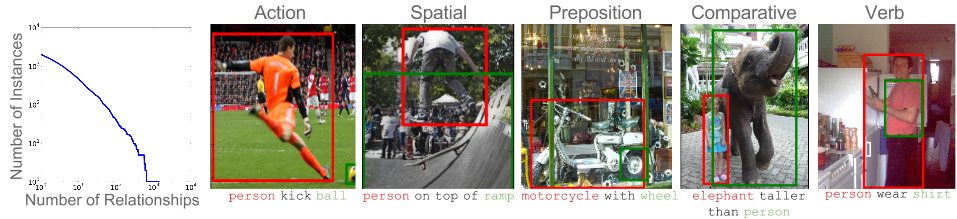
\includegraphics[width=8.8cm]{figures/predica.png}
    \caption{Predicates categorized. Source \cite{Cewu}.}
    \label{fig:predaCar}
\end{figure}

Based on the above, We use the spatial predicates for object characterization, 
since the objects belongs to certain human occupation space, 
such as a room, are static. Whereas, in this case, 
predicates based on verbs (actions) were not useful. In the Figures from 
\ref{fig:abelow} to \ref{fig:topUnder} the relationships used to make the 
knowledge graph are shown.
% Con base en lo anterior, en este trabajo se realizó la caracterización de 
% objetos por medio de predicados espaciales, puesto que los objetos que se 
% encuentran en un determinado espacio de ocupación humana, como una habitación, 
% son estáticos. Mientras que, para este caso, los predicados basados en verbos 
% (acciones) no fueron de utilidad. En las Figuras de \ref{fig:abelow} al 
% \ref{fig:topUnder} se muestran las relaciones que se utilizaron para elaborar 
% el grafo de conocimiento.

\begin{figure}[H]
    \centering
    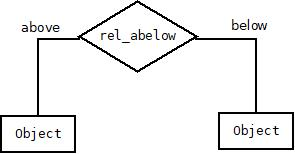
\includegraphics[width=5cm]{figures/abelow.jpg}
    \caption{Relation above-below.}
    \label{fig:abelow}
\end{figure}

\begin{figure}[H]
    \centering
    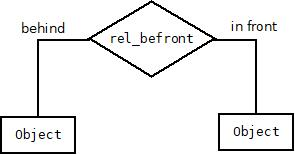
\includegraphics[width=5cm]{figures/befront.jpg}
    \caption{Relation behind-inFront.}
    \label{fig:befront}
\end{figure}

\begin{figure}[H]
    \centering
    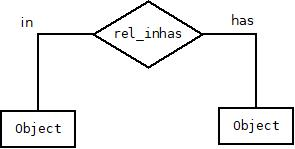
\includegraphics[width=5cm]{figures/inhas.jpg}
    \caption{Relation in-has.}
    \label{fig:inhas}
\end{figure}

\begin{figure}[H]
    \centering
    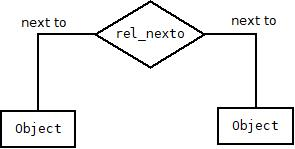
\includegraphics[width=5cm]{figures/nextto.jpg}
    \caption{Relation nextTo.}
    \label{fig:nexto}
\end{figure}

\begin{figure}[H]
    \centering
    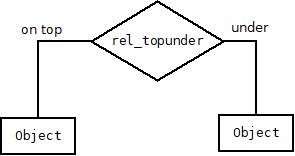
\includegraphics[width=5cm]{figures/topunder.jpg}
    \caption{Relation onTop-under.}
    \label{fig:topUnder}
\end{figure}

The elements recognize as objects have two attributes which are the identifier 
(ID) and the name as shown in Figure \ref{fig:object}. However, as more 
predicates are incorporated, it is possible to add more attributes to the 
object in order to better describe the relationship.
% Los elementos reconocidos como objetos tienen dos atributos los cuales son 
% el identificador (ID) y el nombre como se puede ver en la Figura 
% \ref{fig:object}. Sin embargo, a medida que se vayan incorporando más 
% predicados es posible añadir al objeto más atributos con el fin de describir 
% mejor la relación.


\begin{figure}[H]
    \centering
    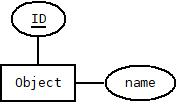
\includegraphics[width=4cm]{figures/object.jpg}
    \caption{Object attributes.}
    % \caption{Atributos de un objeto.}
    \label{fig:object}
\end{figure}

Before implementing the knowledge graph with Grakn, we drafted it, 
to visually identify the relationships that must be created through 
the tool. This conceptual design is seen in Figure \ref{fig:grafo}.
% Antes de implementar el grafo de conocimiento a través de Grakn, se realizó 
% un bosquejo del mismo con la finalidad de identificar de manera visual las 
% relaciones que se deben crear a través de la herramienta. Este diseño 
% conceptual se observa en la Figura \ref{fig:grafo}.

\begin{figure}[H]
    \centering
    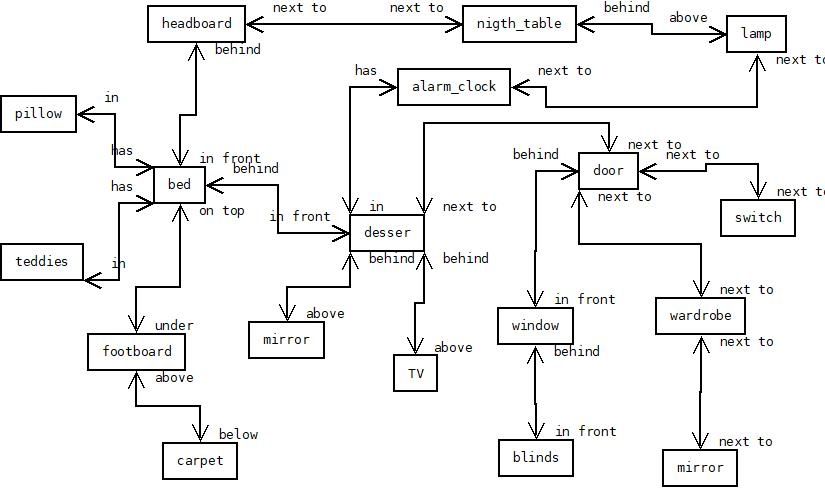
\includegraphics[width=8.8cm]{figures/grafo.jpg}
    \caption{Conceptual design of the knowledge graph.}
    \label{fig:grafo}
\end{figure}

\subsection{Development}
% \subsection{Desarrollo}

The implementation of the knowledge graph in Grakn was based on the previously 
defined relationships scheme, shown in the previous section. Thus, with the 
help of the Graql language, relations of type \texttt{above-below} were defined 
first and then the object, as can be seen in Listing \ref{lst:script1} and 
\ref{lst:script2}, respectively.
% La implementación del grafo de conocimiento en Grakn fue con base en el 
% esquema de las relaciones previamente definidas, mostradas en la sección 
% anterior. Así, con la ayuda del lenguaje Graql se definieron primero las 
% relaciones de tipo \texttt{above-below} y posteriormente el objeto, como 
% se puede ver en Listing \ref{lst:script1} y \ref{lst:script2}, 
% respectivamante.

\lstinputlisting[language=Python, firstline=1, lastline=8,
    caption=Relationship definition using Graql.,
    label={lst:script1}
]{code/schema.gql}
% caption=Definición de las relaciones en 
% Graql,label={lst:script1}]{code/schema.gql}

\lstinputlisting[language=Python, firstline=22, lastline=35,
caption=Object definition using Graql., label={lst:script2}]{code/schema.gql}
% caption=Definición del objeto en Graql,label={lst:script2}]{code/schema.gql}

Later, another script was created to insert the objects, as well as to insert 
the relationships that exist between them. It should be noted that the 
identifier is assigned automatically, so it is not necessary to declare 
it when inserting it. The insertion of the objects is done with the reserved 
word \textit{insert} and the relations with the combination of words 
\textit{insert} and \textit{match}, as seen in Listing \ref{lst:script3} and 
\ref{lst:script4}. A total of seventeen objects were inserted.
% Posteriormente, se creó otro script para insertar los objetos, así como 
% para insertar las relaciones que existen entre éstos. Cabe destacar que el 
% identificador se asigna de manera automática, por lo que, es necesario 
% declararlo a la hora insertarlo. La inserción de los objetos se realiza con 
% la palabra reservada \textit{insert} y las relaciones con la combinación de 
% palabras \textit{insert} y \textit{match}, como se observa en Listing 
% \ref{lst:script3} y \ref{lst:script4}. Se insertaron un total de diecisiete 
% objetos.\\

\lstinputlisting[language=Python, firstline=1, lastline=2,
caption=Object insertion., label={lst:script3}]{code/data.gql}
% caption=Inserción de objetos,label={lst:script3}]{code/data.gql}

\lstinputlisting[language=Python, firstline=62, lastline=65,
caption=Object relationship., label={lst:script4}]{code/data.gql}
% caption=Relación entre los objetos,label={lst:script4}]{code/data.gql}

On the other side, to execute the code it was necessary to create a dedicated 
\textit{keyspace}, which was named \texttt{vision\_relationships}, where the 
schemes and relationships were made. Finally, to check that the objects have 
been inserted correctly, a query was made via console, as shown in Figure 
\ref{fig:correct}. Thus, the created objects were also counted.
% Por otra parte, para ejecutar el código fue necesario crear un 
% \textit{keyspace} dedicado, al cual se nombró \texttt{vision\_relationships}, 
% donde se crean los esquemas y las relaciones mencionadas. Finalmente, para 
% corroborar que los objetos hayan sido insertados correctamente se hizo una 
% consulta vía consola, como se muestra en la Figura \ref{fig:correct}. Así, 
% además se contabilizaron los objetos creados.

\begin{figure}[H]
     \centering
     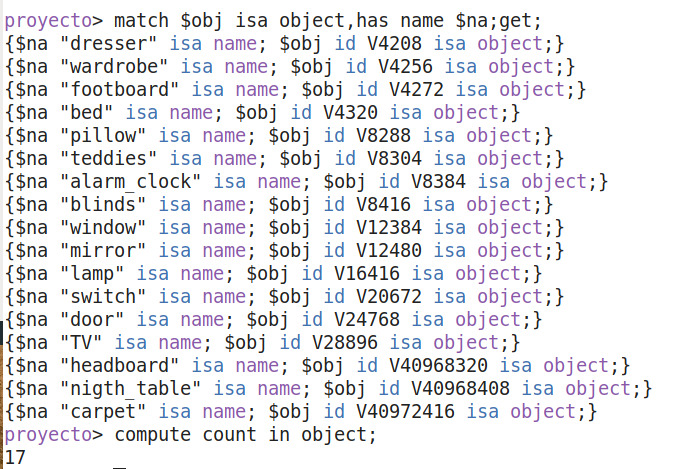
\includegraphics[width=8.8cm]{figures/numObje.jpeg}
     \caption{Query to check that there are no errors.}
    %  \caption{Consulta para corroborar que no existan errores.}
     \label{fig:correct}
\end{figure}